\documentclass[10pt,aspectratio=1609]{beamer}
\usepackage{hyperref}
\usepackage{amsmath}

% \usetheme{CambridgeUS}
\usepackage{aneotheme}


\begin{document}
\author{Jérôme Gurhem}
\title{Cloud computing with \\ ArmoniK}
\subtitle{CSMA Juniors 2025}
\institute{Aneo}
\date{\today}

\titlepage

\AtBeginSection[]
{
	\frame{\sectionpage}
}

\begin{frame}
	\frametitle{Outline}
	\large
	\tableofcontents
\end{frame}

\begin{section}{Our expertise @Aneo}
  \begin{frame}
    \frametitle{Who are we ?}
    \begin{itemize}
      \item Consulting agency specialized in digital transformation
      \item Support for organizational transformations
      \item Assistance in carrying out advanced IT projects
      \item 150 employees
      \item HPC/HTC R\&D team of $\sim$30 people, including 15 PhDs
    \end{itemize}
  \end{frame}

  \begin{frame}
    \frametitle{Technical expertise}
    \begin{itemize}
      \item Code optimization
      \begin{itemize}
        \item Performance analysis and bottleneck identification
        \item Porting applications to support accelerators (Nvidia and AMD GPUs, Google TPU, AWS Trainium, FPGA\dots)
        \item Application industrialisation (automation, reliability, repeatability)
        \item Floating point stabilisation and optimization
      \end{itemize}
      \item Cloud computing
      \begin{itemize}
        \item Application migration to a specific or hybrid cloud provider (AWS, GCP, S3NS, OVH, Qarnot, Oracle\dots)
      \end{itemize}
    \end{itemize}
  \end{frame}

  \begin{frame}
    \frametitle{Floating Point Arithmetic}
    \begin{itemize}
      \item Interflop/FPT4 ANR project with:Aneo, CEA - LIST, EDF, Intel, Sorbonne Université - LIP6, Triscale-Innov, Université Perpignan - LAMPS, UVSQ - Li-PaRAD
      \item Analyzing round-off error propagation in numerical applications
      \item ANEO's contribution:
      \begin{itemize}
        \item Development of PENE
        \item Stochastic Arithmetic: modification of rounding errors in every FP operation
        \item Delta Debug: locate the source of the instabilities in the source code
        \item Dynamic Compilation: based on Intel PIN
        \item Portability: x86 on Linux and Windows
      \end{itemize}
    \end{itemize}
  \end{frame}
\end{section}

\begin{section}{Our vision of Cloud Computing}
  \begin{frame}
    \frametitle{What is the Cloud?}
      \begin{alertblock}{Definition}
      \begin{quote}
        Paradigm for enabling network access to a \textbf<2>{scalable} and \textbf<2>{elastic} pool of shareable physical
        or virtual resources with \textbf<2>{self-service} provisioning and administration \textbf<2>{on-demand}.
        \\
        --- ISO/IEC 17788:2014
      \end{quote}
    \end{alertblock}

    \only<2>{All of that through APIs and code}
  \end{frame}

  \begin{frame}
    \frametitle{Fundamental Principles}
    \centering
    \vfill
    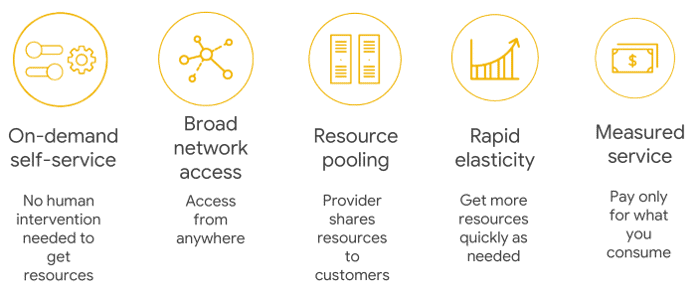
\includegraphics[width=\textwidth]{cloud-fundamentals.png}
  \end{frame}

\begin{frame}
  \frametitle{Cloud Service Models}
  \centering
  \vfill
  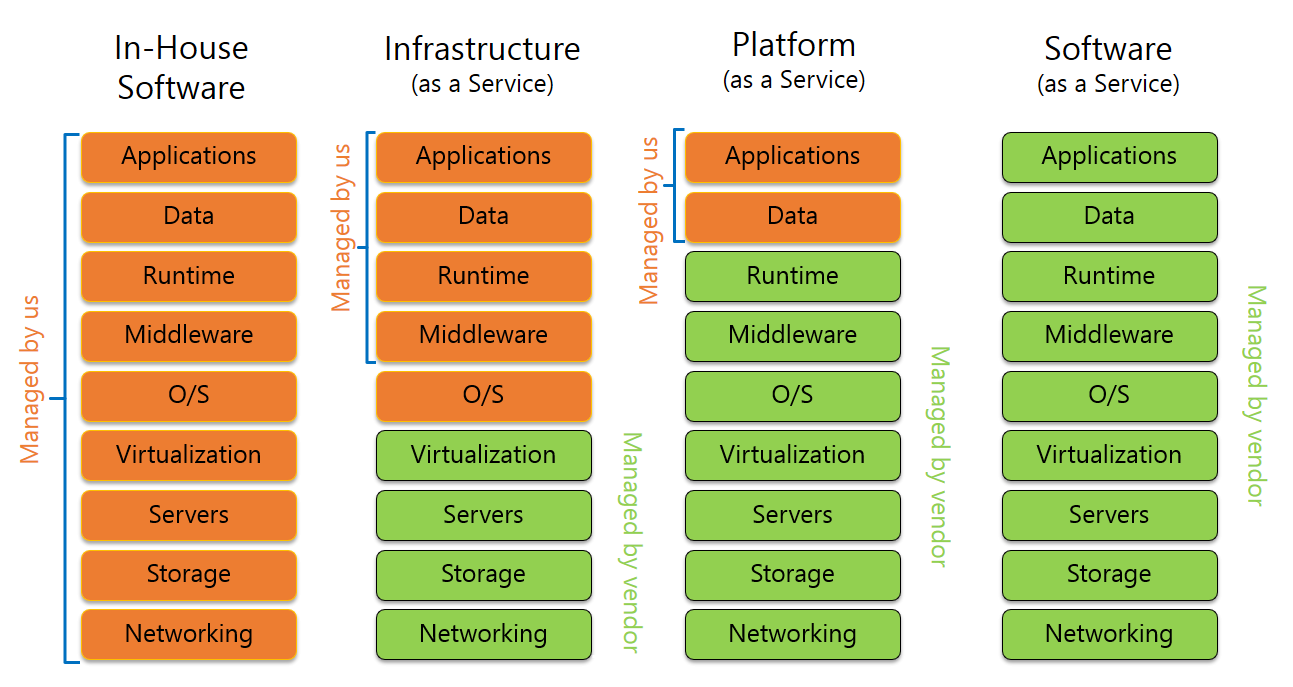
\includegraphics[width=\textwidth]{saas.png}
\end{frame}

% \begin{frame}
%   \frametitle{Scale of Computations}

%   \begin{columns}[T] % Align columns at the top
%     \begin{column}{0.33\textwidth}
%       \textbf{Small scale computations}
%       \begin{itemize}
%         \item Fit on developers' laptop
%         \item Possible need for parametric study
%       \end{itemize}
%     \end{column}
%     \begin{column}{0.33\textwidth}
%       \textbf{Medium scale computations}
%       \begin{itemize}
%         \item Tend to fit on 1 node with 100s of cores
%         \item Previously based on MPI+X and a few nodes
%         \item No longer needed due to single node performance
%         \item Possible need for parametric study
%       \end{itemize}
%     \end{column}
%     \begin{column}{0.33\textwidth}
%       \textbf{Large scale computations}
%       \begin{itemize}
%         \item 100s of nodes
%         \item Tight coupling
%         \item Need for low latency network for good performance
%         \item Based on MPI+X
%       \end{itemize}
%     \end{column}
%   \end{columns}

  % \vspace{1cm}
  % \centering
  % \begin{tikzpicture}[remember picture]
  %   \draw[aneoorange, ->, ultra thick]
  %     ([xshift=0.2\textwidth]current page.west) --
  %     ([xshift=-0.2\textwidth]current page.east)
  %     node[midway, below] {Technical evolution};
  % \end{tikzpicture}
% \end{frame}

% \begin{frame}
%   % todo: verify this slide
%   % ethernet should be checked
%   \frametitle{Large Scale Computations}

%   \begin{itemize}
%     \item \textbf{On-premises}
%     \begin{itemize}
%       \item SLURM, Torque, Moab
%       \item HPC clusters / supercomputers
%       \item High-speed interconnects (InfiniBand, Omni-Path)
%     \end{itemize}

%     \item \textbf{Amazon Web Services (AWS)}
%     \begin{itemize}
%       \item Managed services : AWS Batch, AWS ParallelCluster (SLURM)
%       \item Colocated resources with high-speed ethernet (Elastic Fabric Adapter from AWS)
%       \item Limited to the configurations exposed by AWS
%       \item Useful to start quickly
%     \end{itemize}

%     \item \textbf{Google Cloud Platform (GCP)}
%     \begin{itemize}
%       \item Managed service : Google Batch
%       \item Colocated resources with high-speed ethernet (Google Cloud's high-speed network) --> Falcon
%       \item Aneo contributes on High Availability for GCP SLURM deployment available in Cluster Toolkit
%       \item More configuration options but should be deployed by the user (vs managed services)
%     \end{itemize}
%   \end{itemize}
% \end{frame}


% \begin{frame}
%   \frametitle{1st Game Changers: Single Node Performance}

%   % machines devenues plus puissantes
%   % code devenu plus efficaces et rapides

%   \begin{itemize}
%     \item \textbf{2x AMD EPYC 9965}
%     \begin{itemize}
%       \item AVX512: 16 FP64 operations per cycle
%       \item 192 cores and 384 threads
%       \item 10.3 TFLOPS in FP64
%       \item Allowed to have 2 on the same node
%       \item $\Rightarrow$ 384 \textbf{cores} on the same node!
%     \end{itemize}

%     \item \textbf{NVidia H series GPU}
%     \begin{itemize}
%       \item XXX cuda cores
%       \item 67 TFLOPS in FP64 and 4 PFLOPS in FP8 on tensor cores
%       \item Allowed to have 8 on the same node
%       \item \href{https://nvdam.widen.net/s/nb5zzzsjdf/hpc-datasheet-sc23-h200-datasheet-3002446}{datasheet doc}
%     \end{itemize}
%   \end{itemize}

%   \begin{block}{Impacts}
%     \begin{itemize}
%       \item Scale of computations is changing with time
%       \item Applications used to run on a few nodes can now run on a single node
%       \item Most powerful nodes cost more than 10s of thousands of euros
%     \end{itemize} 
%   \end{block}

% \end{frame}


% \begin{frame}
%   \frametitle{2nd Game changers: Cloud Providers}

%     \begin{itemize}
%       \item Buying powerful machines without fully using them is too expensive
%       \item Available on-demand and pay-as-you-go on the Cloud
%       \item Affordable to use them for computations
%     \end{itemize}

%     \begin{block}{Impacts}
%       \begin{itemize}
%         \item Renting a powerful node for a few hours is better than buying it
%         \item Easy way to get heterogeneous resources (mix of CPUs and GPUs)
%       \end{itemize}
%     \end{block}
% \end{frame}

% \begin{frame}
%   \frametitle{3rd Game changers: Parametric studies}

%   \begin{itemize}
%     \item Small unitary runs
%     \item Needs a lot of them for exploring the parameter space or for Monte-Carlo simulations
%     \item Pre-processing and post-processing of potentially different nature and machines requirements
%     \item $\Rightarrow$ graph of hybrid computations
%     \item May be large scale computations at the end
%   \end{itemize}
% \end{frame}

% \begin{frame}
%   \frametitle{Challenge: Fault Tolerance}

%   \begin{itemize}
%     \item Preemptible: cheaper (up to 80\%) computing resources that can be interrupted and reclaimed by the cloud provider anytime
%     \item Applications must be able to recover from failures and continue execution
%     \item Not suitable for all applications
%     \item Large scale MPI-based applications not designed to handle loss of nodes
%     \begin{itemize}
%       \item Checkpointing and Restart is the main strategy
%       \item Can work for preemptible resources but there is no guarantee that all the nodes will be available for the application to execute
%       \item PMIx not fully supported for addition and removal of nodes during application execution
%     \end{itemize}
%     \item Very suitable for graph of small scale computations
%     \begin{itemize}
%       \item Application can be reexecuted on another node if a preemption occurs
%       \item Support for heterogeneous resources
%       \item Adapt to the available resources count
%     \end{itemize}
%   \end{itemize}
% \end{frame}


% \begin{frame}
%   \frametitle{How to take advantage of these features ?}

%   \begin{itemize}
%     \item Computations nature is changing with AIs and hardware evolutions
%     \item Cloud introduces new computing paradigms for computations and hardware accessibility
%     \item Decoupling of application and infrastructure lead to Serverless computing
%   \end{itemize}
% \end{frame}


\begin{frame}
  \frametitle{Supercomputers vs Cloud Computing}

    \begin{itemize}
      \item Both give access to a large number of interconnected computing resources
      \item Both have persistent storage
      \item Both provide job scheduling and resource management
      \item Execute a job and rent cloud resources for a few hours is similar
      \item Using supercomputers is very close to using a cloud provider
    \end{itemize}

    \begin{block}{Main differences}
      \begin{itemize}
        \item Cloud is general purpose
        \item Cloud offers more diverse services
        \item From a user perspective, Cloud resources are almost unlimited
      \end{itemize}
    \end{block}
\end{frame}


\begin{frame}
  \frametitle{HPC = Grand Challenge ?}


  \begin{columns}[T] % Align columns at the top
    \begin{column}{0.5\textwidth}
      \textbf{2007}
      \begin{itemize}
        \item JUGENE \textbf{Supercomputer}
        \item 222 TFlops
      \end{itemize}
      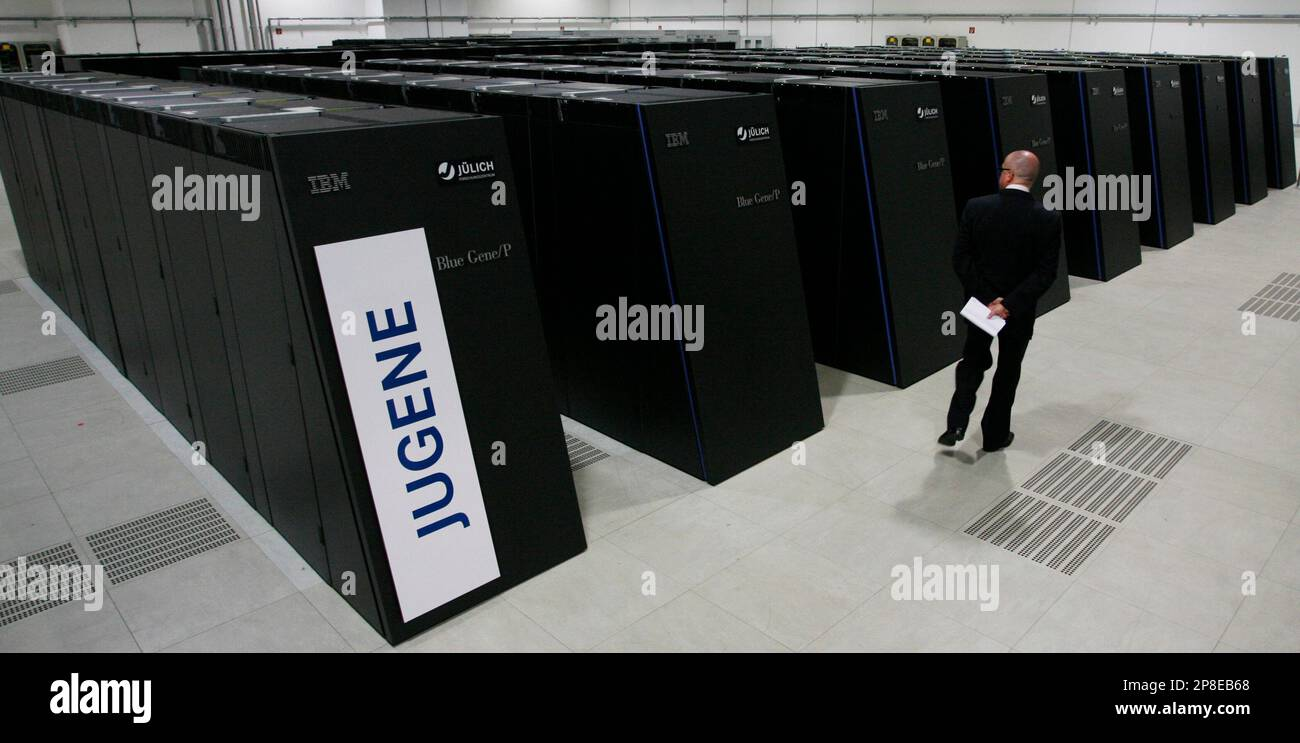
\includegraphics[width=0.95\textwidth]{supercomputer-jugene.jpg}
    \end{column}
    \begin{column}{0.5\textwidth}
      \textbf{2025}
      \begin{itemize}
        \item 2025 Nvidia GB200 \textbf{chip}
        \item 160 TFlops

      \end{itemize}
      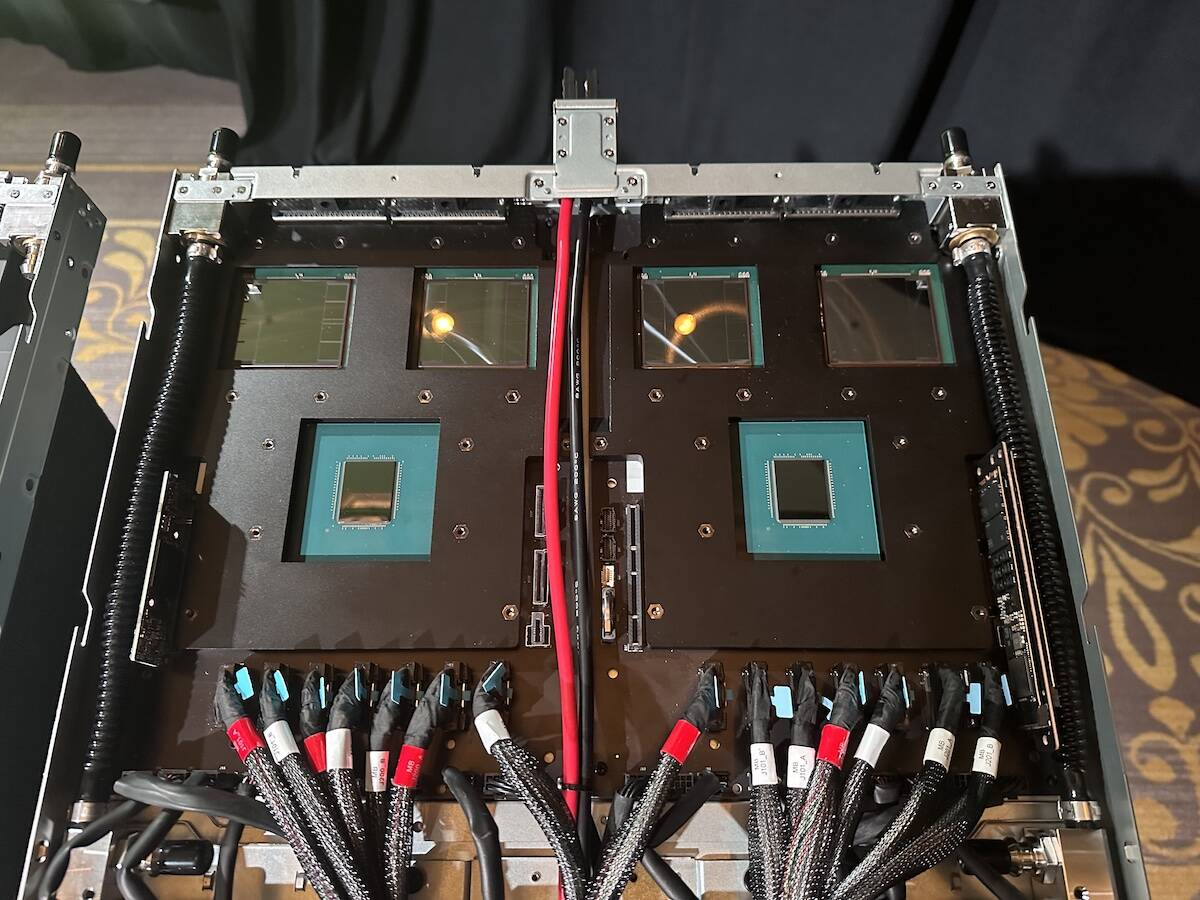
\includegraphics[width=0.95\textwidth]{chip-gb200.png}
    \end{column}
  \end{columns}

    % Ajouter la slide avec la comparaison des perfs avec 20 ans écart
    \begin{block}{Impacts}
      \begin{itemize}
        \item Supercomputers from 15 years ago are a single node today
      \end{itemize}
    \end{block}
\end{frame}


\begin{frame}
  \frametitle{Yesterday's use cases have become commodities}

  \begin{itemize}
    \item Past large scale computations are now a building block for applications
    \begin{itemize}
      \item Part of optimization algorithms
      \item Used for training AI models
      \item Multiphysics Coupling
    \end{itemize}

    \item They still need lots of resources
    \begin{itemize}
      \item Many runs with different parameters
      \item Need for pre-processing, aggregation and post-processing of results
      \item Computations can be heterogeneous
      \item Complex coupling and dependencies
    \end{itemize}
  \end{itemize}

\end{frame}

\begin{frame}
  \frametitle{Has HPC become HTC?}

  \begin{block}{HPC}
    Few large communicating jobs 
  \end{block}

  \begin{block}{HTC}
    Lots of small independant computations 
  \end{block}

  \begin{block}{New Workloads}
    Lots of small computations with dependencies and complex data management

    $\Rightarrow$ Mix between HPC and HTC
  \end{block}

\end{frame}
\end{section}

\begin{section}{ArmoniK: A Bridge Between HPC, HTC and Cloud}
  
  \begin{frame}
    \frametitle{ArmoniK: a Hybrid Framework}
    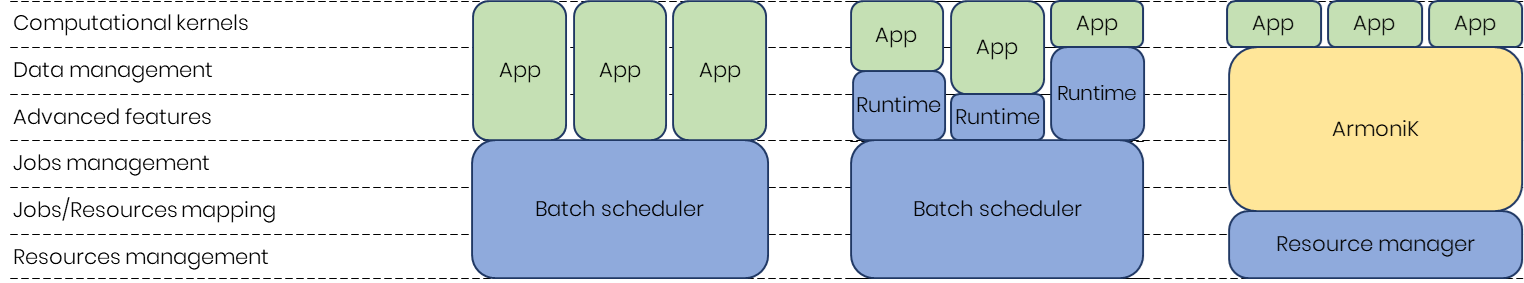
\includegraphics[width=\textwidth]{hpc-orchestrators.png}
    \begin{itemize}
      \item Computational kernels: User computations
      \item Data management: Reads, Writes, Communications between processes
      \item Advanced features: Overlapping, load balancing
      \item Jobs management: Job queues, resource allocation, job lifecycle
      \item Jobs / Resources mapping: Determine job execution on which machines
      \item Resources management: Machine pool update, node addition or removal
    \end{itemize}
  \end{frame}

  \begin{frame}
    \frametitle{A Serverless Many-Task Computing Platform}
    \begin{alertblock}{Serverless}
      \begin{quote}
        Cloud service category in which the customer can use different cloud capabilities types
        without the customer having to provision, deploy and manage either hardware or software
        resources, other than providing customer application code or providing customer data.
        \\
        --- ISO 22123-2:2023
      \end{quote}
    \end{alertblock}
    \begin{alertblock}{Many-Task Computing}
      \begin{quote}
        Approach that aims to bridge the gap between High-Perfomance Computing and High-Throughput Computing.
        \\
        --- Wikipedia
      \end{quote}
    \end{alertblock}
  \end{frame}

  \begin{frame}
    \frametitle{Task-based Programming in ArmoniK}
    \begin{block}{Definition}
      Paradigm focusing on the decomposition of complex operations into smaller tasks
    \end{block}
    \begin{itemize}
      \item Expression of complex data-driven dependencies
      \item ArmoniK's \textbf{distributed scheduler} responsible for:
      \begin{itemize}
        \item Task distribution and load balancing
        \item Dependency resolution
        \item Tasks execution
        \item Data management (overlapping, prefetching, and checkpointing)
      \end{itemize}
    \end{itemize}
  \end{frame}

  \begin{frame}
    \frametitle{ArmoniK Programming Model}
    \begin{columns}[T]
      \begin{column}{0.5\textwidth}
        \begin{itemize}
          \item \textbf{Task Graph}: Bipartite DAG whose node sets are tasks and data
          \item \textbf{Task node}: Single-node computation (possibly multi-threaded) taking one or several data inputs and outputting one or several data
          \item \textbf{Data node}: Immutable piece of data depending on only one task at most
          \item \textbf{Dependencies}: Dependencies between tasks are expressed as data dependencies
          \item \textbf{Dynamic}: The graph may not be entirely known in advance (tasks can append tasks and replace edges with subgraphs)
        \end{itemize}
      \end{column}
      \begin{column}{0.5\textwidth}
        \centering
        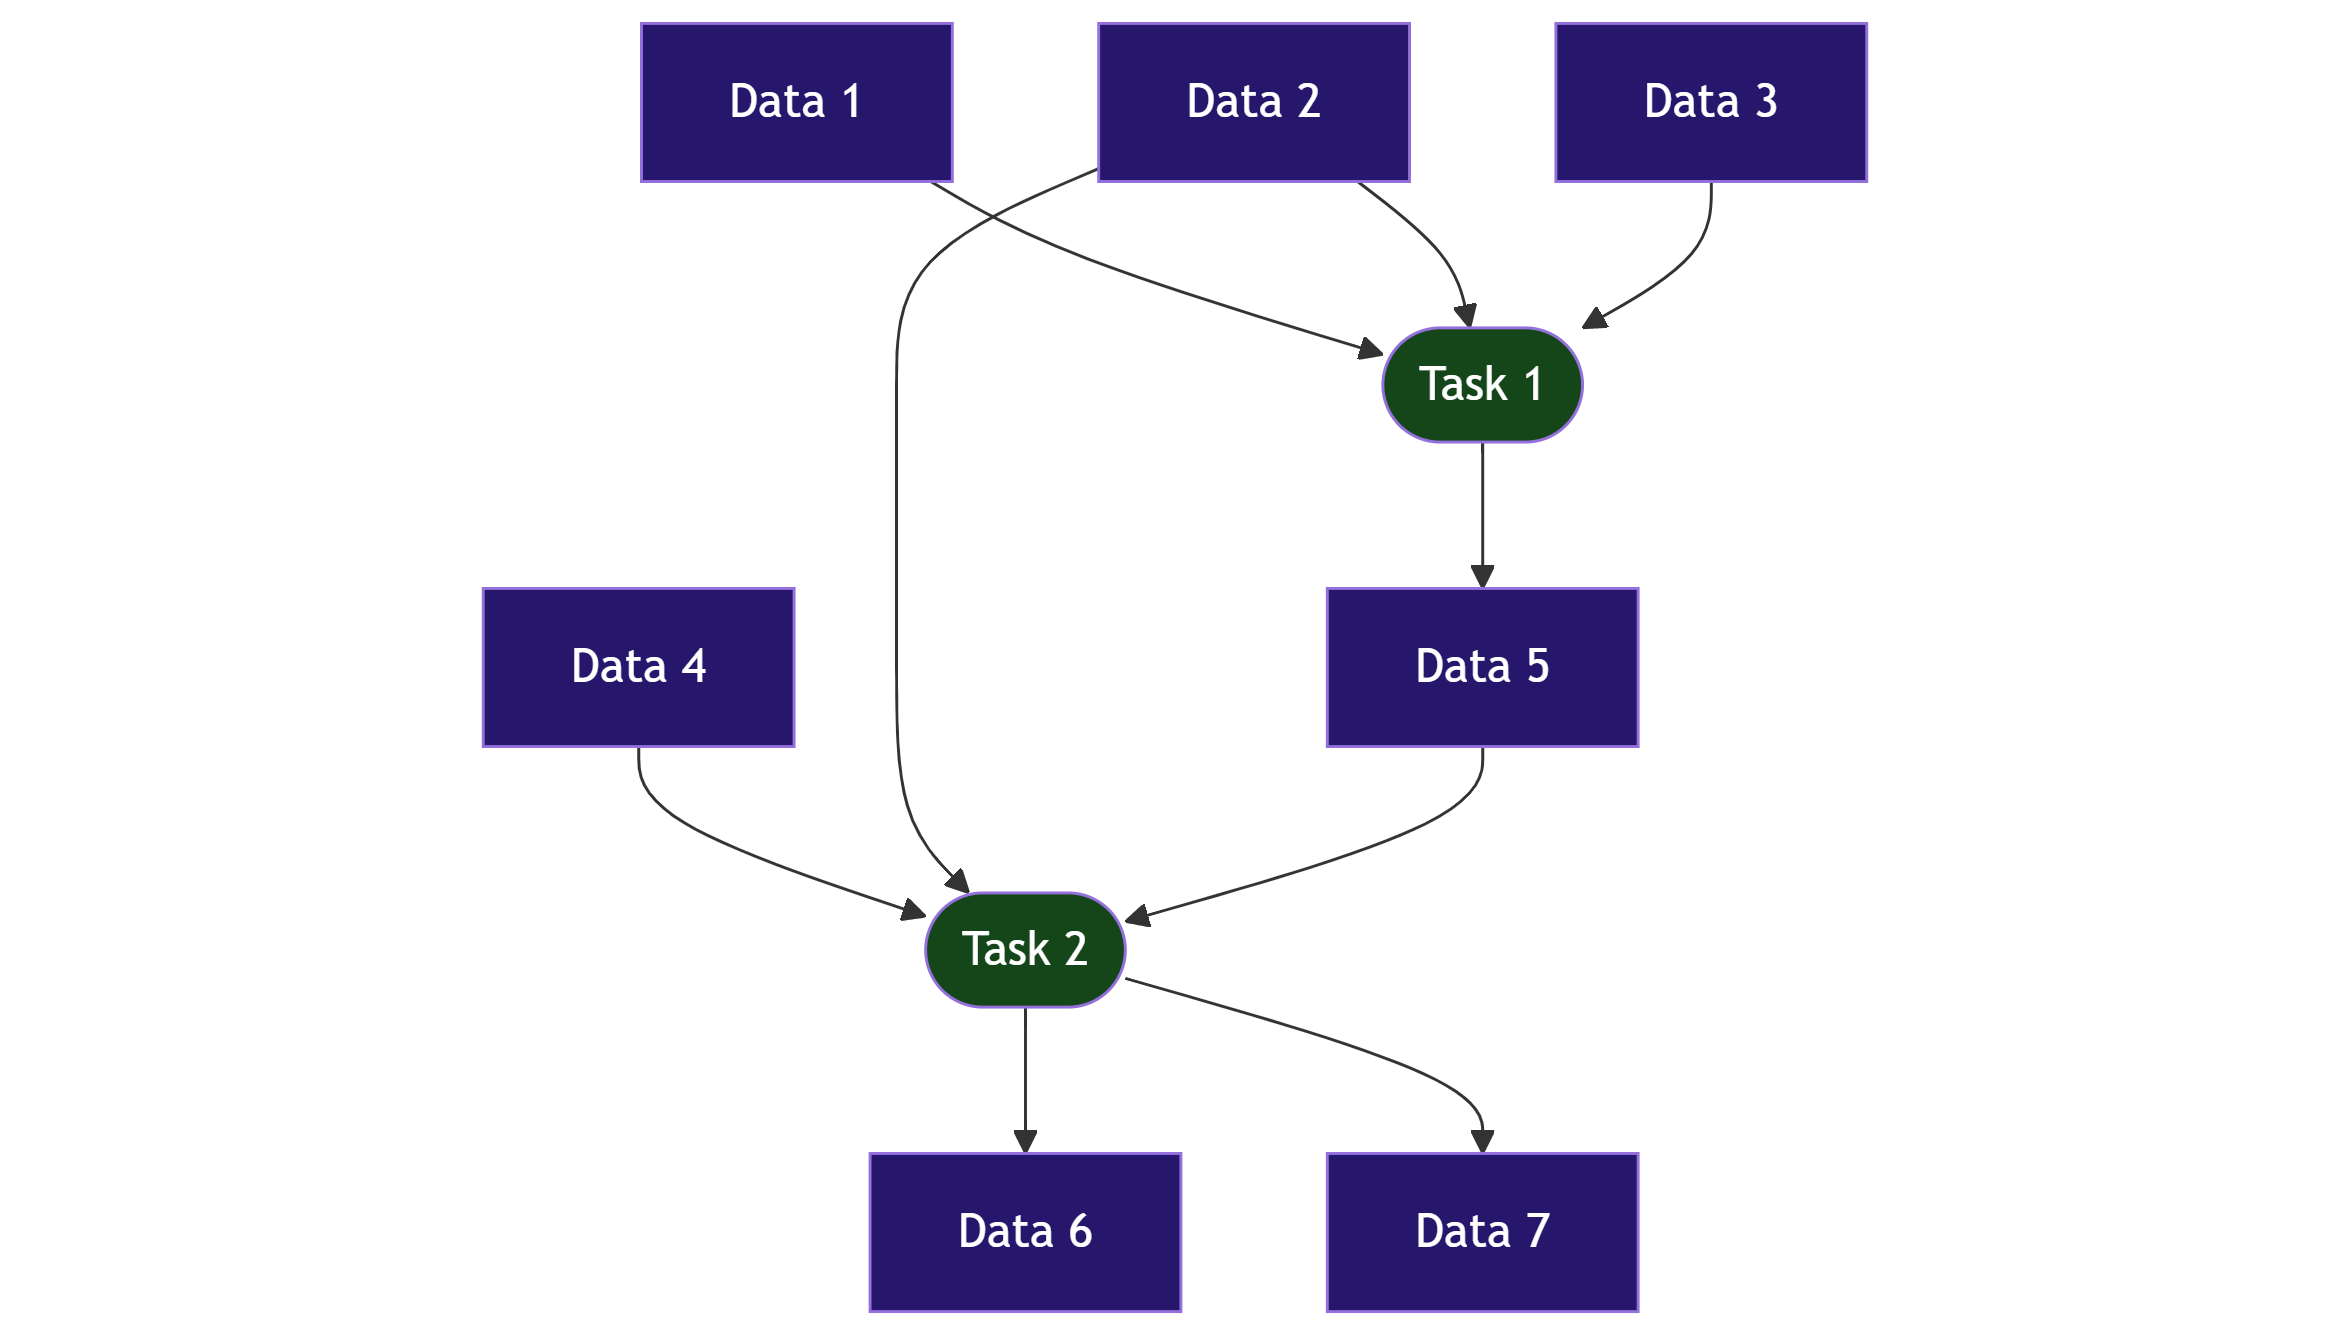
\includegraphics[width=0.95\textwidth]{mermaid-task-graph.png}
      \end{column}
    \end{columns}
  \end{frame}

  \begin{frame}
    \frametitle{The Client-Worker Pattern}
    \begin{columns}[T]
      \begin{column}{0.5\textwidth}
        \begin{itemize}
          \item \textbf{Client}: User-developed software that submits the initial task graphs to ArmoniK and retrieves results
          \item \textbf{Worker}: User-developed software capable of performing one or several tasks, depending on its implementation:
          \begin{itemize}
            \item Can take input data, perform calculations, and return a result
            \item Can submit new tasks and set the result as output of a new task
          \end{itemize}
          \item \textbf{Synchronization via Data}: The client might not be aware that the task graph has been modified
        \end{itemize}
      \end{column}
      \begin{column}{0.5\textwidth}
        \centering
        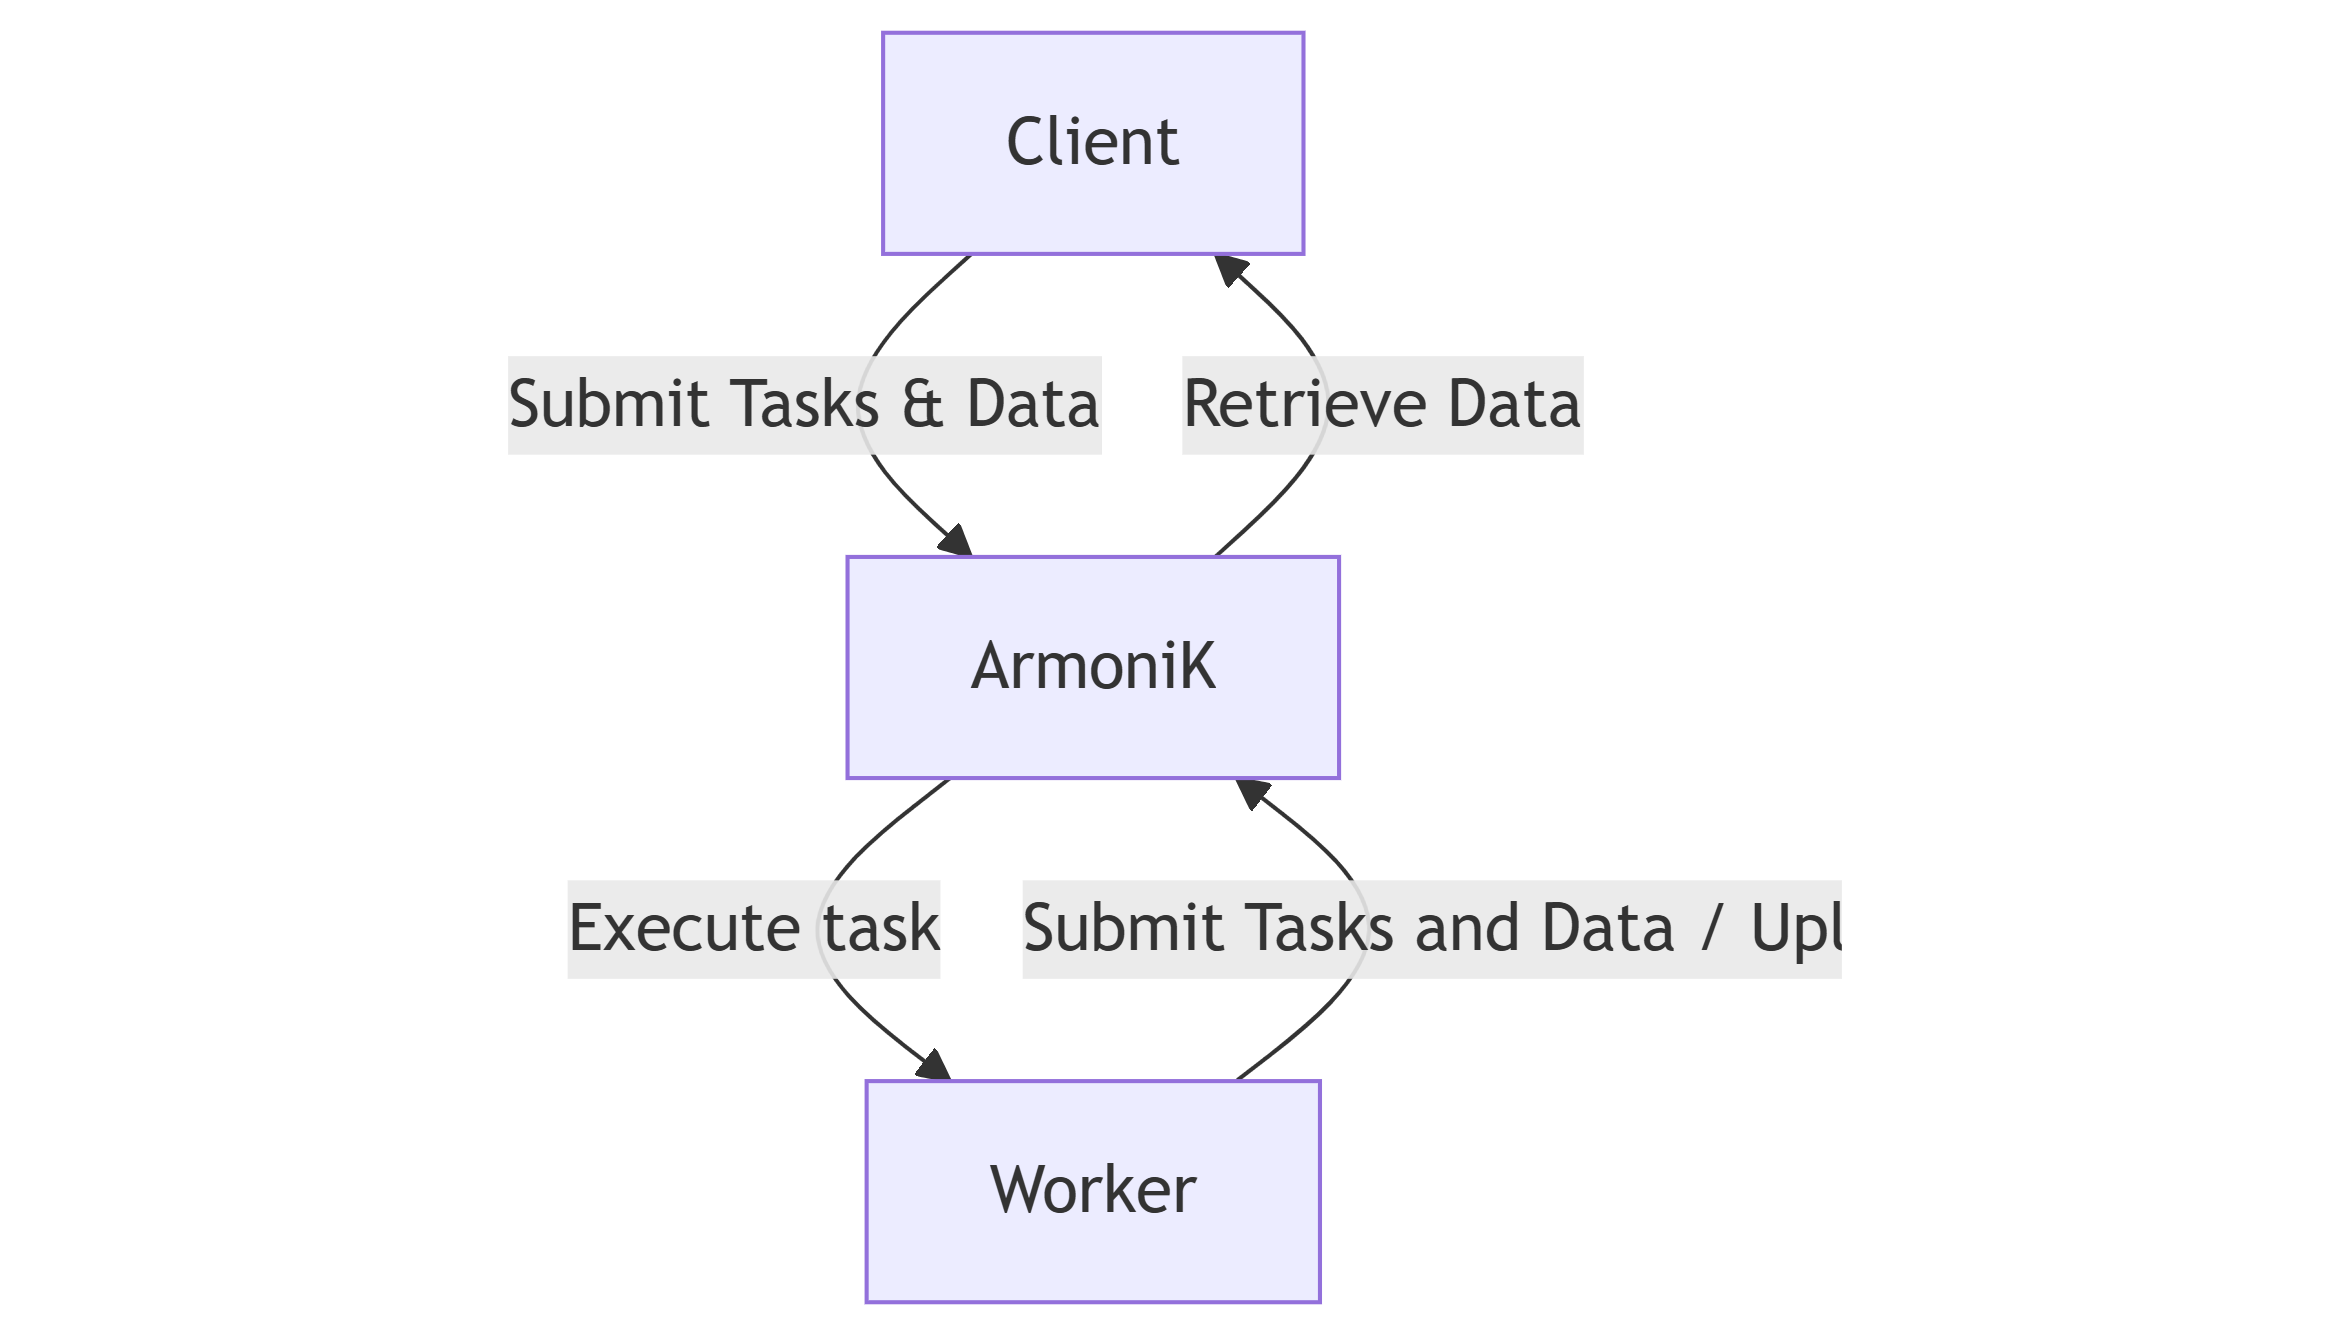
\includegraphics[width=0.95\textwidth]{mermaid-client-worker.png}
      \end{column}
    \end{columns}
  \end{frame}

  \begin{frame}
    \frametitle{Dynamic Graph}
    \begin{block}{Definition}
      Dependency graph is not fully known when scheduling starts.
    \end{block}
    \begin{itemize}
      \item Task dependencies not known before submission
      \item Submissions can happen anytime
      \item Tasks can submit new tasks
      \item Tasks can delegate the production of their output to their new tasks
    \end{itemize}
  \end{frame}

  \begin{frame}
    \frametitle{Dynamic Graph Example}
    \begin{columns}[T]
      \begin{column}{0.3\textwidth}
        \centering
        \vspace{1cm}
        \vfill
        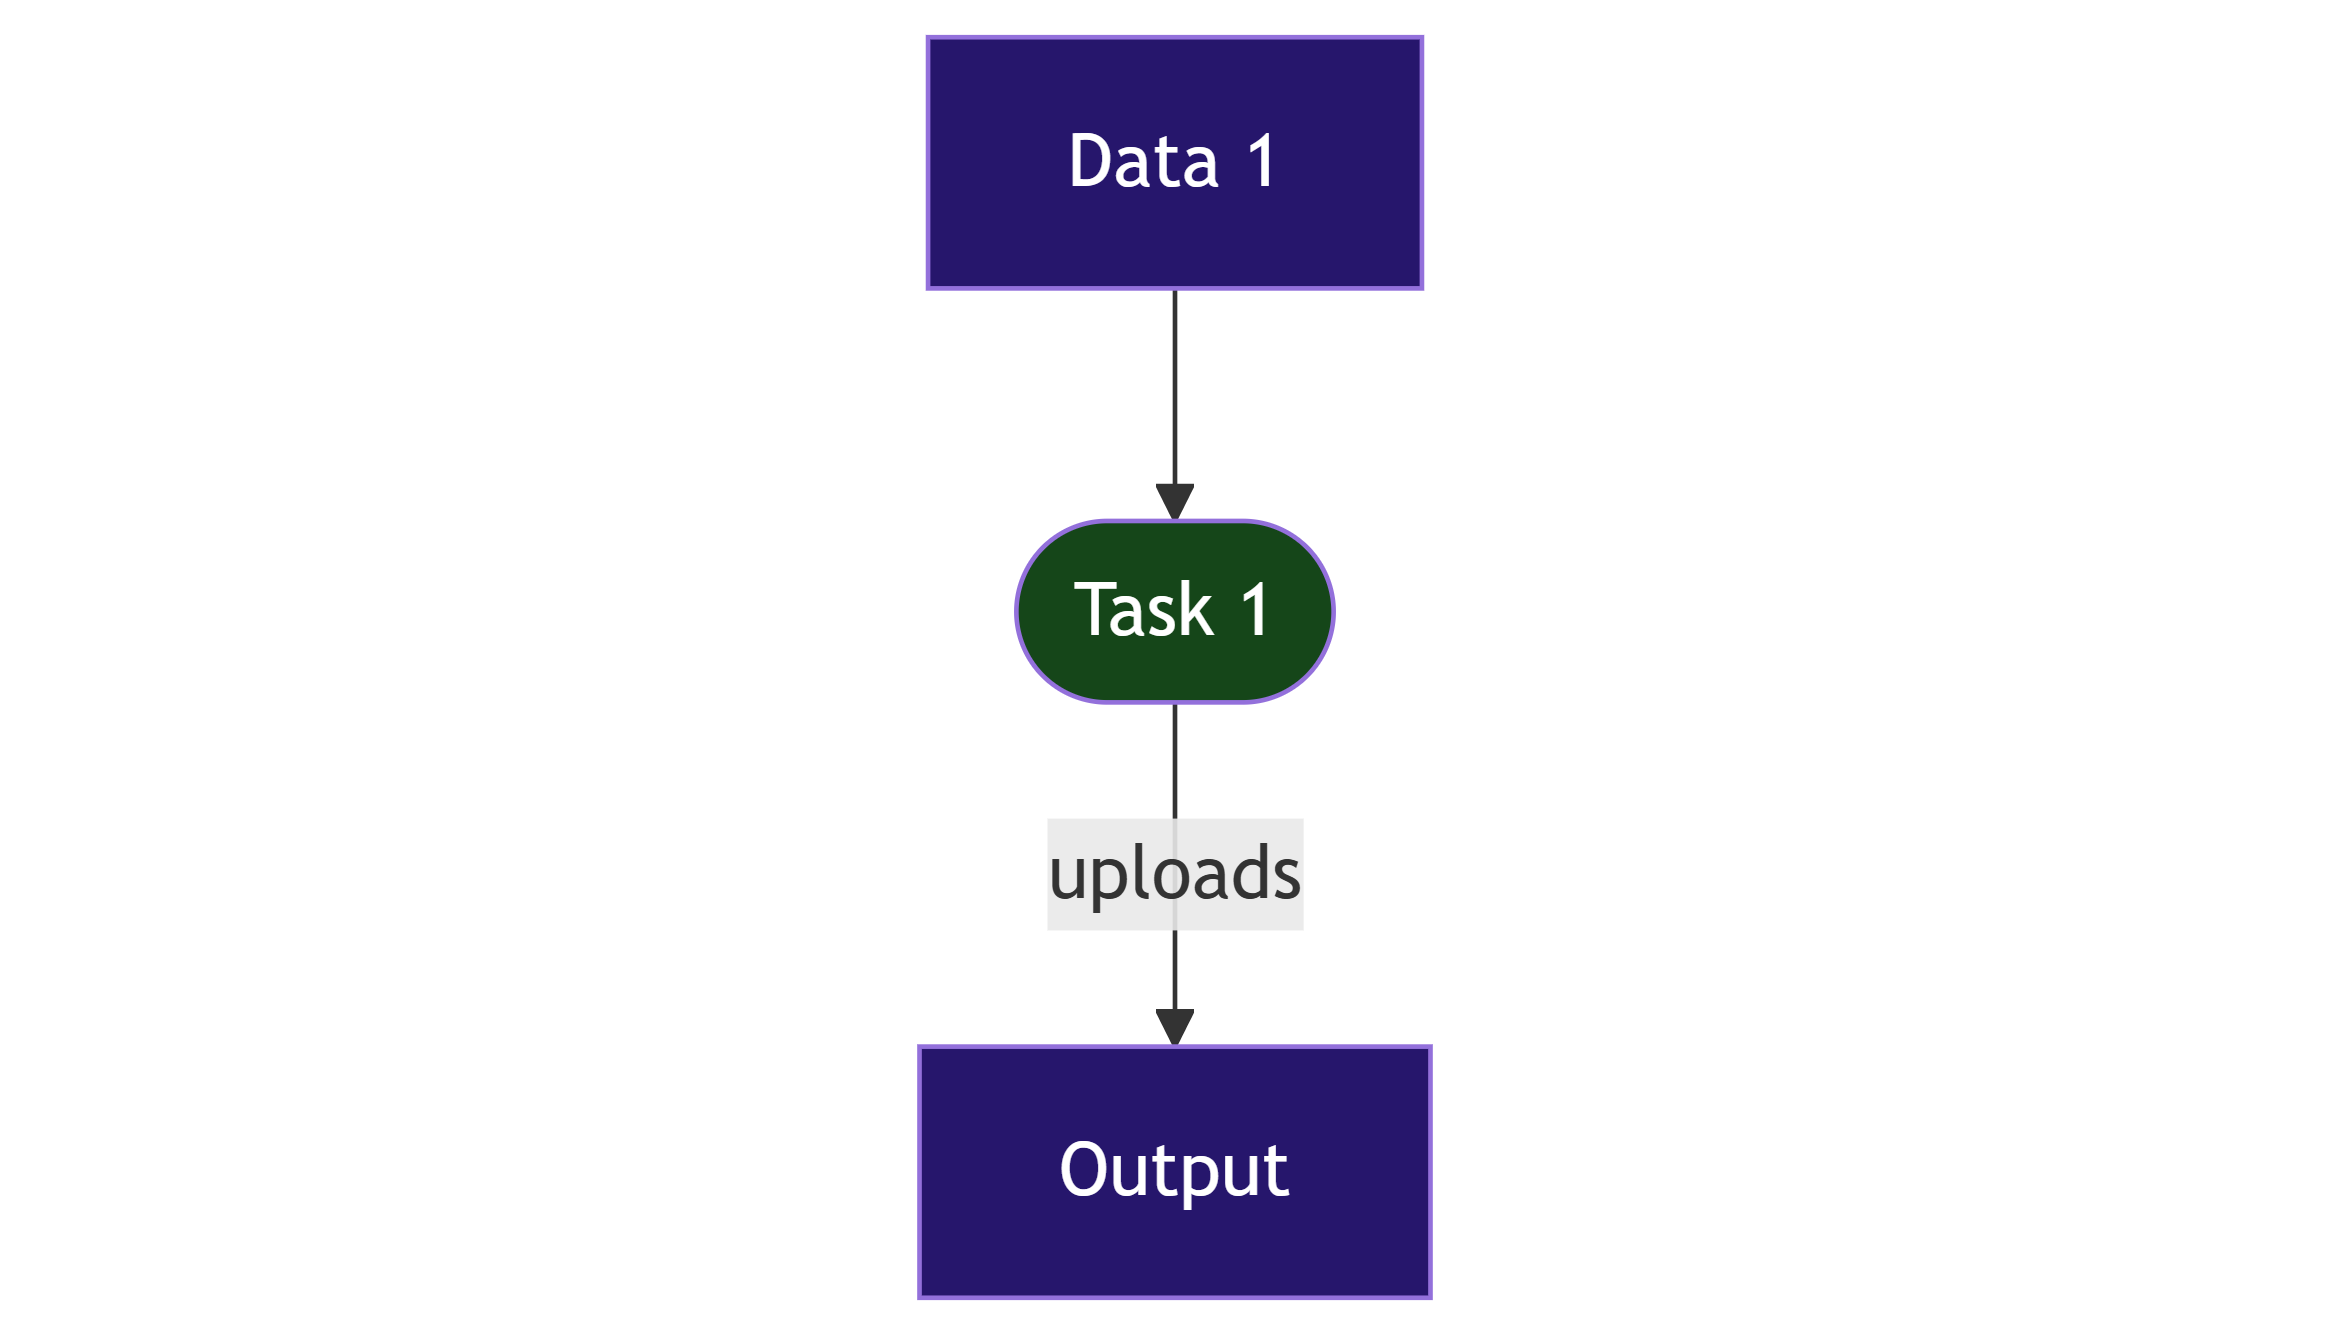
\includegraphics[width=0.95\textwidth]{mermaid-dynamic-part1.png}
      \end{column}
      \begin{column}{0.05\textwidth}
        \centering
        \vspace{1.7cm}
        \vfill
        $\Rightarrow$
      \end{column}
      \begin{column}{0.65\textwidth}
        \centering
        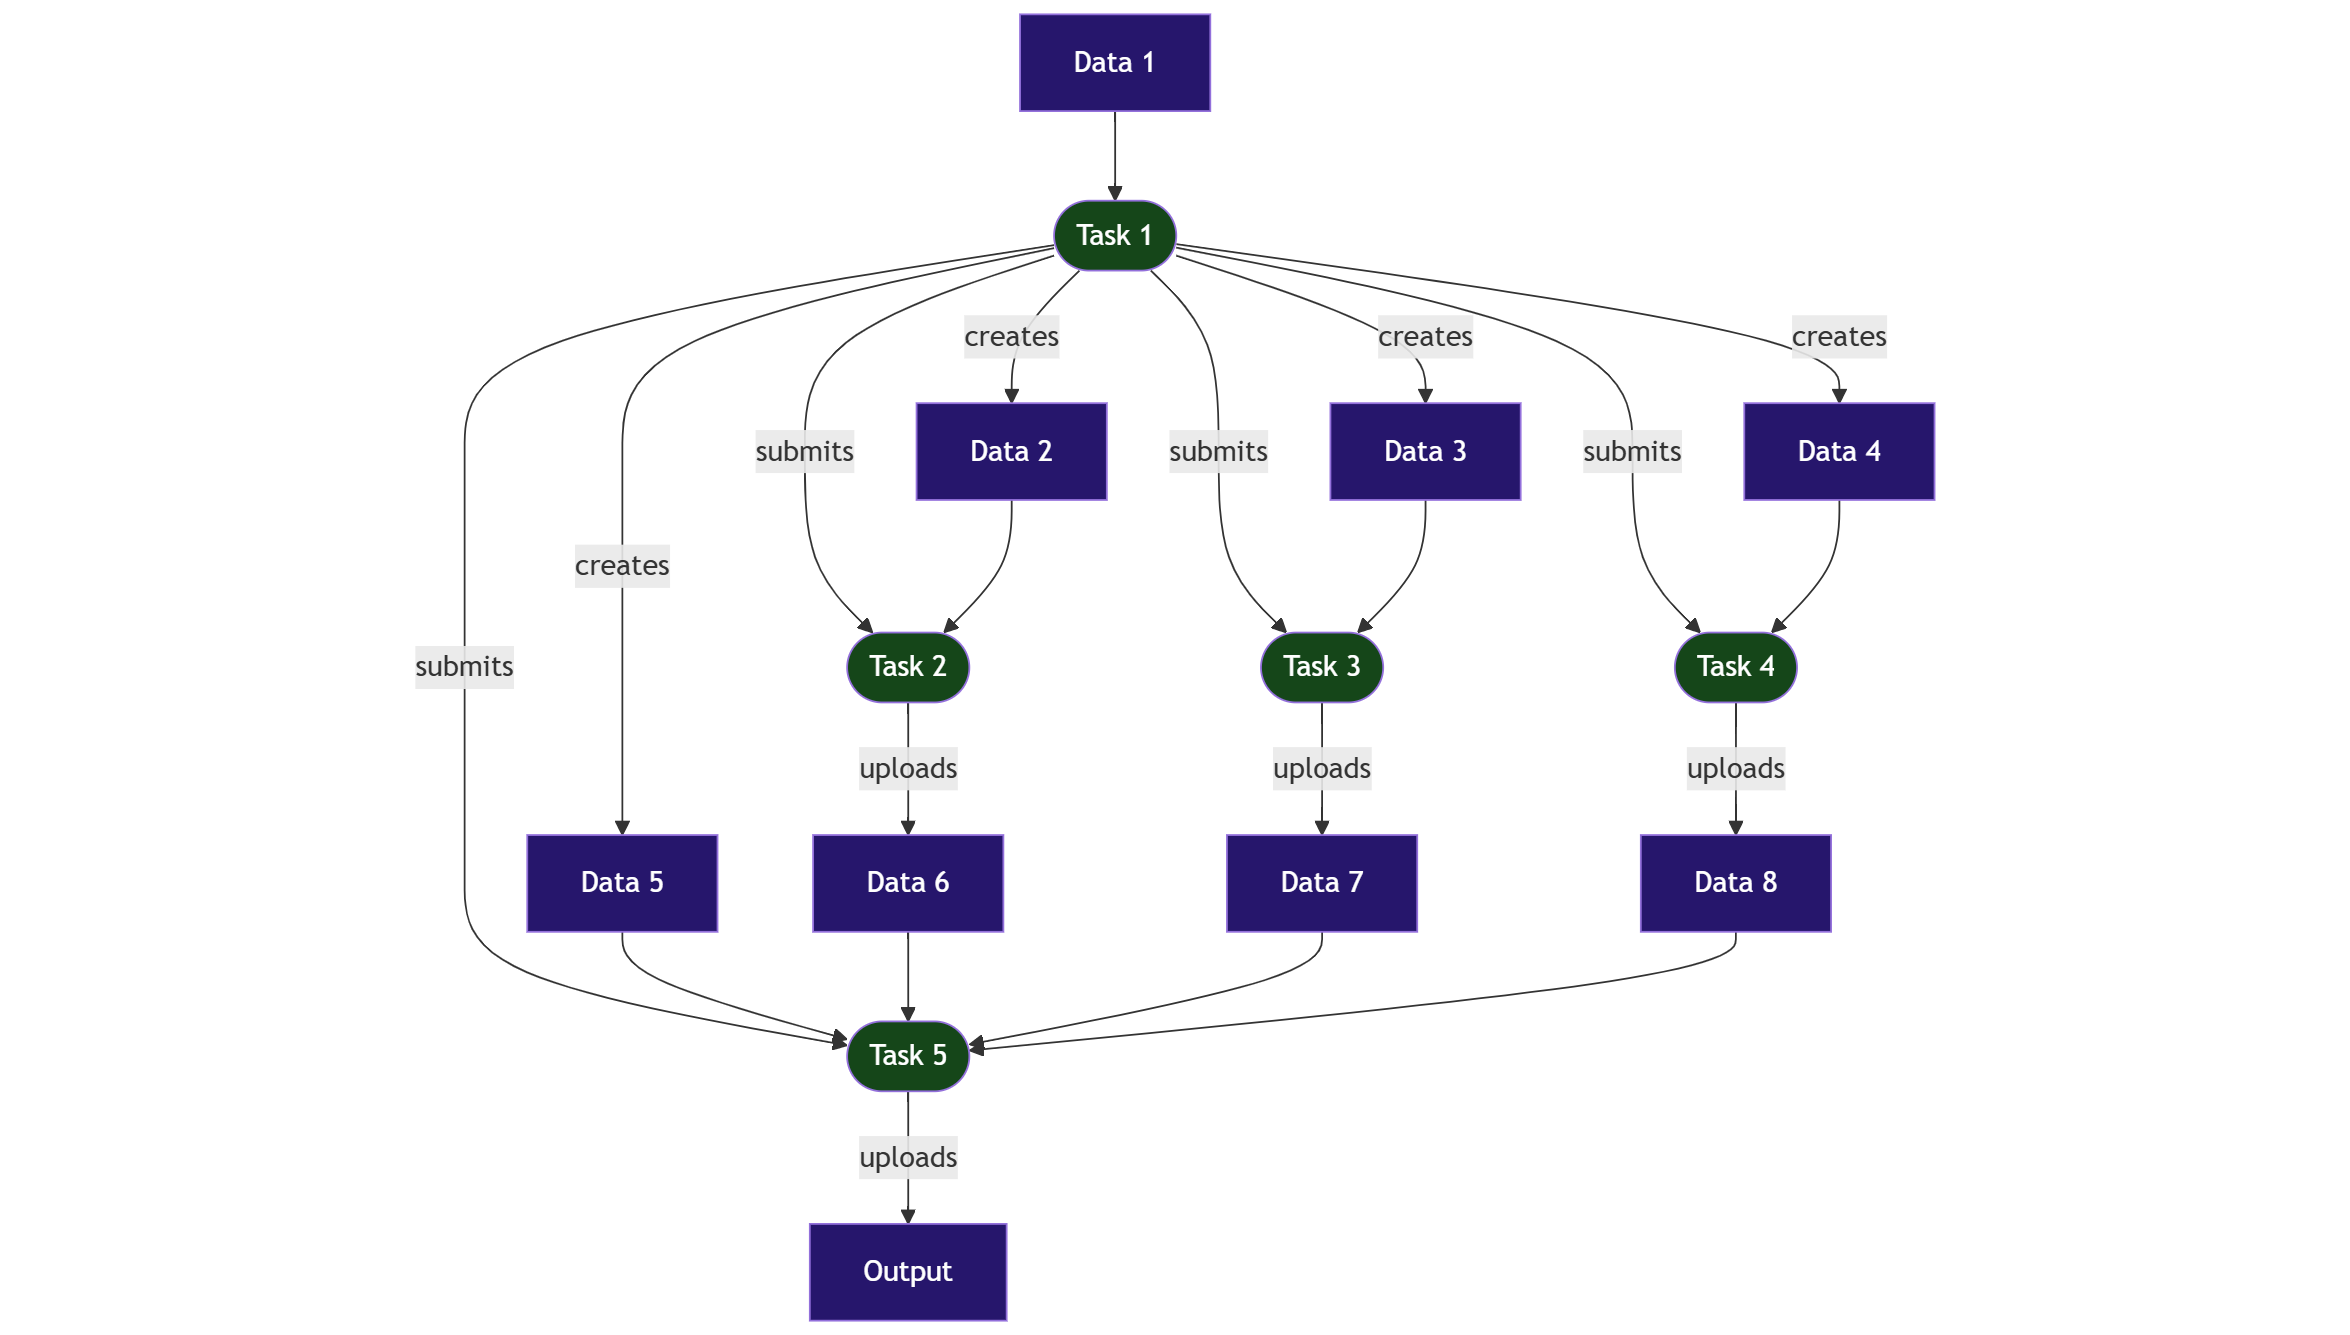
\includegraphics[width=0.95\textwidth]{mermaid-dynamic-part2.png}
      \end{column}
    \end{columns}
  \end{frame}

  \begin{frame}
    \frametitle{Computions/Comm Overlapping}
    \begin{block}{Data Management}
      Responsibility for data allocation, transfer, and storage between computational operations
    \end{block}
    \begin{itemize}
      \item ArmoniK is responsible for tasks input and output data management
      \item Allows for automatic communication + scheduling/task execution overlapping
      \item Automatic Uncoordinated Checkpointing
      \item Data communications through global storage
    \end{itemize}
    % schema pour le pipelining
  \end{frame}

  \begin{frame}
    \frametitle{Observability}
    % mettre la video de Jules
    \begin{block}{Definition}
      Ability to understand the internal state of a system based solely on its external outputs.
    \end{block}
    \begin{itemize}
      \item GUI to monitor workflows and tasks status (optional)
      \item Expose metrics about ArmoniK and tasks states
      \item Tooling to emit, collect and search application/orchestration logs
      \item Provide monitoring APIs that can show tasks and data status
      \begin{itemize}
        \item Available in multiple languages
        \item Can be integrated into monitoring systems
      \end{itemize}
      \item CLI built on top of our APIs
      \begin{itemize}
        \item Can be improved to support more features
        \item We are open to suggestions
      \end{itemize}
    \end{itemize}
  \end{frame}

  \begin{frame}
    \frametitle{ArmoniK Main Features}
    \begin{itemize}
      \item \textbf{Portability}: Effort to transfer an application from one environment to another
      \begin{itemize}
        \item Officially supported languages: C\#, C++, Python, Rust, Java, and JavaScript
        \item Tasks on different architectures (x86, ARM, GPU, Linux, Windows), applications, environments
      \end{itemize}
      \item \textbf{Fault Tolerance}: Ability to continue functioning without interruption when one or more nodes fail
      \begin{itemize}
        \item Allow support for preemptible computing resources
        \item Error management at the task level
      \end{itemize}
      \item \textbf{Malleability}: Dynamic reconfiguration of the number of allocated resources during execution without interruption
      \item \textbf{Resource Sharing}: Share resources between applications to execute as many as possible at the same
      \item \textbf{Modularity}: Modules can be swapped without modifying ArmoniK's code to suit user neeeds and constraints
    
    \end{itemize}
  \end{frame}

  \begin{frame}
    \frametitle{Production in Critical Systems}
    \begin{block}{Definition}
      System that meets all functional and non-functional requirements, is thoroughly tested, and is stable, secure, scalable, and maintainable enough to be deployed in a live production environment.
    \end{block}
    \begin{itemize}
      \item In production!
      \item Used by our clients in their critical systems
      \item Explains our needs for:
      \begin{itemize}
        \item Validation and guarantees
        \item Monitoring
        \item Stability
      \end{itemize}
    \end{itemize}
  \end{frame}

\end{section}

\begin{section}{How can we make ArmoniK address more data intensive applications ?}

  \begin{frame}
    \frametitle{Data-Aware Scheduling Strategies}
    \begin{itemize}
      \item Current scheduling
      \begin{itemize}
        \item Dependencies resolution managed by ArmoniK
        \item Tasks distribution done by the queue system (contains only tasks with dependencies available)
      \end{itemize}
      \item Improvements
      \begin{itemize}
        \item Affinity task-data
        \begin{itemize}
          \item Schedule tasks to the agent where inputs are in cache or close
          \item Colocate sub-graphs with common dependencies
        \end{itemize}
        \item Fine-grained data lifecycle management
        \begin{itemize}
          \item Caching system to store data on the nodes
          \item Data usage hints to help remove data from cache when not used anymore
          \item Data can be used as dependencies during new tasks submission (dynamic graph)
          \item Help scheduler during task distribution and checkpointing
        \end{itemize}
      \end{itemize}
    \end{itemize}
  \end{frame}

  \begin{frame}
    \frametitle{Supercomputer Deployment}
    \begin{itemize}
      \item Kubernetes not available on most supercomputers
      \item Needs an alternative resource manager for ArmoniK
      \begin{itemize}
        \item Run ArmoniK within a SLURM job
        \item More advanced integration with SLURM
        \begin{itemize}
          \item Use SLURM as ArmoniK resource manager
          \item Take advantage of SLURM queues to run ArmoniK compute plane
        \end{itemize}
      \end{itemize}
      \item Docker not available too
      \begin{itemize}
        \item Docker rootless
        \item Singularity
      \end{itemize}
      \item Need tests and integration in order to validate it works properly
      \item Done by HPC-Whisk
    \end{itemize}
  \end{frame}

  \begin{frame}
    \frametitle{Performance Analysis Tools}
    \begin{itemize}
      \item Usually a complex task due to the complexity of the problem solved and the software stack
      \item Increased complexity with ArmoniK's malleability making the number of resources used vary
      \item Provide data usable for performance analysis
      \item Build tooling to allow users to easily identify performance bottlenecks
    \end{itemize}
  \end{frame}

  \begin{frame}
    \frametitle{Formal Validation of ArmoniK's Properties}
    \begin{itemize}
      \item Quentin's PhD goal
      \item Modelize ArmoniK scheduler
      \item Validate scheduling is fault tolerant, efficient, and malleable
    \end{itemize}
  \end{frame}

  \begin{frame}
    \frametitle{We are looking for other use cases}
    \begin{itemize}
      \item Today, we mainly have financial applications
      \item We are also working in integrating AI tools
      \item We study autonomous driving solutions with an automotive industrial
      \item We need more use cases
        % couplage -> acceleration de methodes iteratives avec de l'IA, deux applications par taches
        % subtasking -> methodes particulaires : radioprotection, lagrangien, ray tracing
      \item Maybe yours !
    \end{itemize}
  \end{frame}

\end{section}

\begin{section}{Are you interested in our solution ? $\rightarrow$ Come next session}
  \begin{frame}
    \frametitle{Open source project}
    \begin{itemize}
      \item ArmoniK code is fully available on github
      \item \href{https://github.com/aneoconsulting/ArmoniK}{ArmoniK's GitHub}
      \item You can contribute
      \item We are open to collaborations
      \item How to use it ?
      \begin{itemize}
        \item \href{https://armonik.readthedocs.io/en/latest/content/armonik/getting-started.html}{Getting started}
      \end{itemize}
    \end{itemize}
  \end{frame}

  \begin{frame}
    \frametitle{Next session}

    Come use ArmoniK with us!

  \end{frame}

  \begin{frame}
    \frametitle{Thank you for your attention!}
    Questions?
  \end{frame}
\end{section}

\end{document}